\documentclass[../report.tex]{subfiles}
\begin{document}
\graphicspath{{img/}{../img/}}

\section{The Waterfall Model}

The waterfall model is a process model which follows a sequence of phases working from the top to the bottom. It is also known as the one-shot or once-through model, because of the non-iterative workflow. The model exists in different versions, but it often consists of five predefined phases. That is \textit{Requirements}, \textit{Design}, \textit{Implementation}, \textit{Verification} and \textit{Maintenance}.

\begin{figure}[H]
\centering
	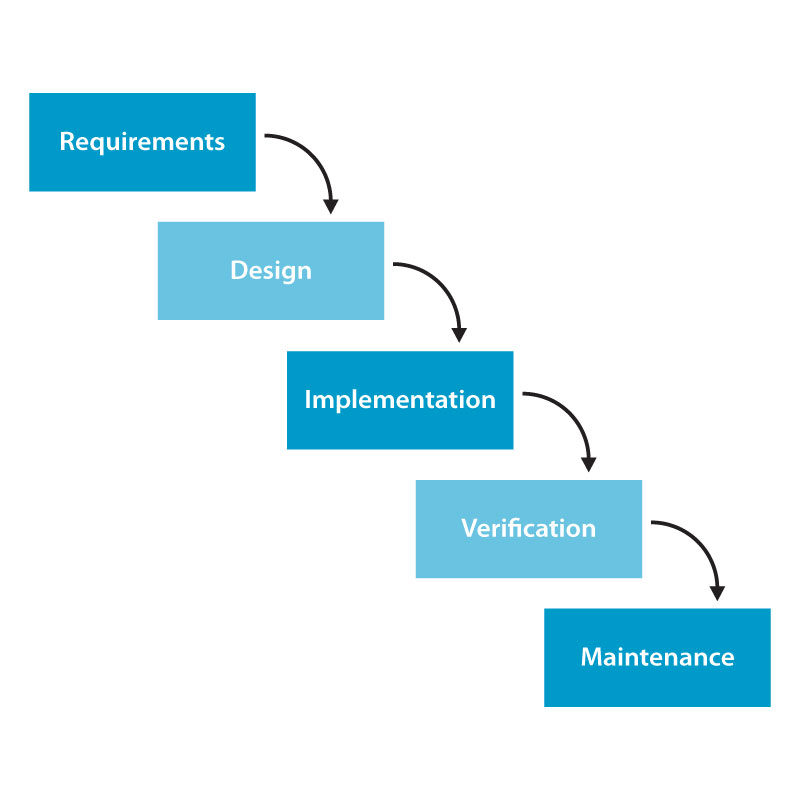
\includegraphics[scale=0.3]{h4_waterfall.jpg}
\caption{The Waterfall Model}
\end{figure}

The flow of the model should always be downwards, however the possibility of ``splashing'' back to the previous phase is allowed. This is more the exception than the rule.

\subsection{Strengths \& Weaknesses}
The strict flow of this process model gives a very limited scope for iteration. This limited scope is indeed a strength, if the requirements of the project are well defined. The progress of the project is easy to follow, both for developers, project managers and the client, since the end of each phase generates a natural milestone for the project. Because of this it is easy to evaluate on the current progress and estimation of the remainder of the project after each phase.

As said The Waterfall Model is preferred if the requirements are well defined, and that no more requirements will be added on later in the process. Because of the non-iterative workflow, there is no way to implement new requirements along the way, it is simply not allowed. The model is generally inflexible, due to the permanent dealings for each phase.
 
Another weakness would be the integration of the product, and the possibility for the client to try the product during the project.

\end{document}